\subsection{Stability analysis}
\begin{frame}{Linear advection equation of an arbitrary quantity $q$}%{One-dimensional problems}
  \begin{block}{Scheme equation (finite difference sense)}
    \begin{footnotesize}
      \begin{equation*}
        \bar{q}^{p,n+1}=\sum_{k=1}^{N_p}H_{pk}(\vect{X}^p,\vect{X}^k,\text{CFL})\bar{q}^{k,n}
      \end{equation*}
    \end{footnotesize}
  \end{block}
  \begin{block}{von-Neumann linear stability analysis}
    \begin{footnotesize}
      The numerical scheme is stable if:
      \begin{equation*}
        \sum_{k=1}^{N_p}\abs{H_{pk}} \leq 1 \quad \forall p
      \end{equation*}
      \alert{$\Rightarrow$ find the maximal CFL number ensuring the stability}
    \end{footnotesize}
  \end{block}\pause
  \metroset{block=fill}
  \begin{footnotesize}
    \begin{block}{Particular case: one particle per cell}
      The first-order FVM is recovered $\rightarrow$ CFL improved compared to MPM 
    \end{block}
    %Comment on CTU + other discretizations
  \end{footnotesize}
  %% Reformuler cette slide sans equation ou alors ecrire le grand principe de minimisation de la fonctionnelle dont l'argument est le CFL pour laisser de la place aux commentaires sur les discrétisations
\end{frame}

\subsection{Convergence analysis}
\begin{frame}
  \begin{block}{\footnotesize Elastic one-dimensional bar -- small strains}
    \begin{columns}
      \begin{column}{0.45\textwidth}
        \centering
        \begin{tikzpicture}
          \draw[thick] (0,0) -- (2,0);
          \draw[pattern=north west lines] (2,-0.25) rectangle (2.25,0.25);
          \draw[->,Red,thick] (-.5,0) node[left] {$\sigma(x=0,t)$} -- (0,0);
          \path (1.,0) edge[bend right] (1.5,-0.5) ;
          \node[right] at (1.5,-0.5) {$E,\rho,l$};
        \end{tikzpicture}
      \end{column}
      \begin{column}{0.45\textwidth}
        $\sigma(x=0,t) = \sigma^d \sin\(\frac{0.4\pi}{l} \sqrt{\frac{E}{\rho}}\:t\)$
      \end{column}
    \end{columns}
  \end{block}
  \begin{overprint}
    \onslide<1>
    %% Graph pour 2ppc regularly spaced
    \begin{block}{\footnotesize $L^2$ relative error -- two particles per cell}
      \begin{columns}
        \begin{column}{0.49\textwidth}
          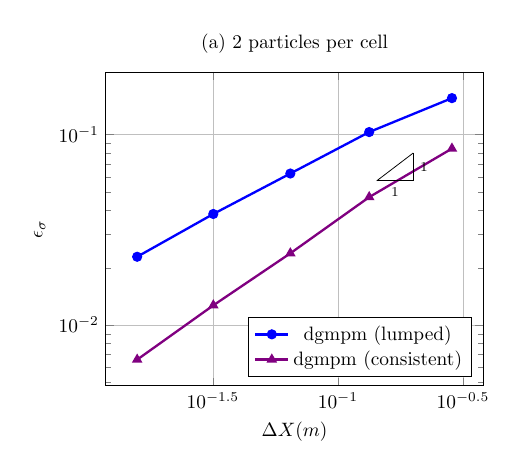
\begin{tikzpicture}[scale=0.7]
\begin{loglogaxis}[xlabel=$\Delta X (m)$,ylabel=$\epsilon_\sigma$,ymajorgrids=true,xmajorgrids=true,legend pos=south east,title={(a) 2 particles per cell}]
\addplot[Blue,very thick,mark=*] coordinates {(0.285714285714,0.155344401413) (0.133333333333,0.103056278416) (0.0645161290323,0.0624467155513) (0.031746031746,0.0383032357895) (0.0157480314961,0.0228383166886) };
\addlegendentry{dgmpm (lumped)}
\addplot[Purple,very thick,mark=triangle*] coordinates {(0.285714285714,0.0844046229439) (0.133333333333,0.0469432859143) (0.0645161290323,0.0238077178296) (0.031746031746,0.0126928564059) (0.0157480314961,0.0065867196308) };
\addlegendentry{dgmpm (consistent)}
\draw (axis cs:0.2,0.08) -- (axis cs:0.2/1.4,0.08/1.4);
\draw (axis cs:0.2,0.08) -- (axis cs:0.2,0.08/1.4) node [midway,right] {\scriptsize 1};
\draw (axis cs:0.2,0.08/1.4) -- (axis cs:0.2/1.4,0.08/1.4) node [midway,below] {\scriptsize 1};
\end{loglogaxis}
\end{tikzpicture}

        \end{column}
        \begin{column}{0.49\textwidth}
          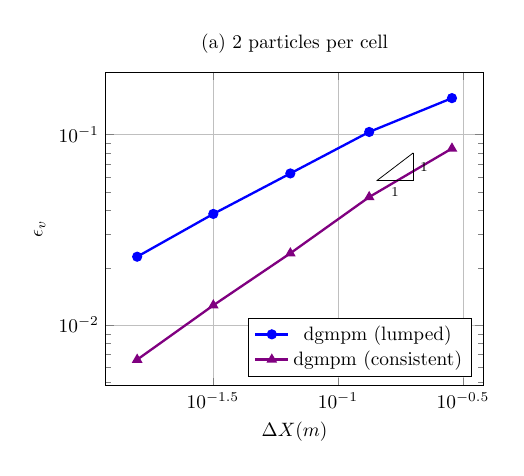
\begin{tikzpicture}[scale=0.7]
\begin{loglogaxis}[xlabel=$\Delta X (m)$,ylabel=$\epsilon_v$,ymajorgrids=true,xmajorgrids=true,legend pos=south east,title={(a) 2 particles per cell}]
\addplot[Blue,very thick,mark=*] coordinates {(0.285714285714,0.155081880585) (0.133333333333,0.103056265942) (0.0645161290323,0.0624467155504) (0.031746031746,0.0383032357895) (0.0157480314961,0.0228383166886) };
\addlegendentry{dgmpm (lumped)}
\addplot[Purple,very thick,mark=triangle*] coordinates {(0.285714285714,0.0844044636359) (0.133333333333,0.0469432859143) (0.0645161290323,0.0238077178296) (0.031746031746,0.0126928564059) (0.0157480314961,0.0065867196308) };
\addlegendentry{dgmpm (consistent)}
\draw (axis cs:0.2,0.08) -- (axis cs:0.2/1.4,0.08/1.4);
\draw (axis cs:0.2,0.08) -- (axis cs:0.2,0.08/1.4) node [midway,right] {\scriptsize 1};
\draw (axis cs:0.2,0.08/1.4) -- (axis cs:0.2/1.4,0.08/1.4) node [midway,below] {\scriptsize 1};
\end{loglogaxis}
\end{tikzpicture}

        \end{column}
      \end{columns}
    \end{block}

    \onslide<2>
    %% Tableau pour les autres
    \begin{block}{\footnotesize $L^2$ relative error -- other space discretizations}
      \centering
      \vskip 10pt
      \begin{footnotesize}
          \begin{tabular}{c|cc|cc|cc|cc}
    \hline
    PPC & \multicolumn{2}{c}{DGMPM--Euler}  \vline & \multicolumn{2}{c}{DGMPM--RK2}\vline  & \multicolumn{2}{c}{MPM} \vline & \multicolumn{2}{c}{MPM--PIC}  \\ [6pt]
    & $\sigma$ & $v$  & $\sigma$ & $v$  & $\sigma$ & $v$ & $\sigma$ & $v$\\ 
    \hline
    \hline
    2 & 0.63 & 0.63 & 0.80 &0.80 & 0.88 & 1.46&0.94& 0.85\\
    6 & 0.66 & 0.66 & 0.91 &0.91 &  0.91&1.62&1.07&0.92\\
    10 & 0.67 & 0.67 & 0.93 &0.93 &0.92&1.62&1.10&0.92\\
    20 & 0.68 & 0.67 & 0.95 &0.95 &0.92&1.61&1.12&0.93\\
    \hline
  \end{tabular}

%%% Local Variables:
%%% mode: latex
%%% TeX-master: "../../mainManuscript"
%%% End:

      \end{footnotesize}
      
    \end{block}
  \end{overprint}
  
\end{frame}

%%% Local Variables:
%%% mode: latex
%%% TeX-master: "../presentation"
%%% End:
